\documentclass[11pt]{amsart}
\usepackage{geometry}                % See geometry.pdf to learn the layout options. There are lots.
\geometry{letterpaper}                   % ... or a4paper or a5paper or ...
%\geometry{landscape}                % Activate for for rotated page geometry
%\usepackage[parfill]{parskip}    % Activate to begin paragraphs with an empty line rather than an indent
\usepackage{booktabs}
\usepackage{graphicx}
\usepackage{amssymb}
\usepackage{epstopdf}
\usepackage{caption}
\usepackage{subcaption}
\usepackage{commath}
\DeclareGraphicsRule{.tif}{png}{.png}{`convert #1 `dirname #1`/`basename #1 .tif`.png}

% Declare commands
\newcommand{\mat}[1]{\mathbf{#1}}

\title{CS 181 -- Practical 3}
\author{Casey Grun, Sam Kim, Rhed Shi}
%\date{}                                           % Activate to display a given date or no date

\begin{document}
\maketitle

% -----------------------------------------------------------------------------
\section{Warmup}


% -----------------------------------------------------------------------------
\section{Classification}

Our challenge was to classify a set of programs, based on traces of their system calls, as either a type of malware or a non-malicious program. Given an $N \times D$ matrix $\mat{X}$ representing the programs, along with a $N$-dimensional vector $\vec{t}$ of training labels, produce a function 
$$y : \mat{X'} \mapsto \vec{t'}$$.
That is, a function which could produce labels $\vec{t'}$ for some matrix $\mat{X'}$. There were two parts to this challenge: determining the \emph{feature functions} to generate rows of the matrix $\mat{X}$ based on the system calls for each malware program, and determining what classification algorithm to use to generate the function $y$.

We developed a cross-validation procedure to test our predictions on folds of the training data before submitting our predictions to Kaggle on the test data; we used 10 folds. A persistent problem we observed was that predicted scores in cross-validation were 0.1--0.2 higher than the scores we recieved on the public leaderboard on Kaggle. We suspect this was because of the heterogeneous training data 

\subsection{Feature Functions}

We evaluated a number of feature functions:
\begin{description}
  \item[System call counts] Our first feature simply summed the number of system calls across all threads in all processes for a particular program. This method achieved ???? on the public leaderboard.
  \item[$n$-grams of system calls] Our most substantial feature examined counts of sequences of system calls. Each unique sequence of $n$ system calls was represented as a feature that counted how many times this sequence appeared in any given malware. We used cross-validation to try and optimize the choice of $n$---the length of these sequences. Too small an $n$ would result in uninformative sequences, while too large an $n$ would not generalize well. We found the optimum $n$ to be approximately 8. 
  \item[DLLs loaded] We also created features counting how many times each unique DLL was loaded with the \verb|load_dll| system call. This feature proved to be reasonably informative, and achieved our best score on Kaggle (in combination with the 8-grams of system calls). 
  \item[Registry keys] Finally, we employed a similar method to count the number of times each unique registry key was read by a program. This feature was less informative than the DLLs or 8-grams, so it was not included in our final predictions.
\end{description}

Additionally, we attemped classification on a reduced-dimensionality feature set, generated by performing a truncated singular value decomposition (TSVD) on the full feature set. This method did not perform particularly well, so it was not pursued. 

Our final/best score was achieved by combining the DLLs, 8-grams, and system call counts features.

\begin{figure}
  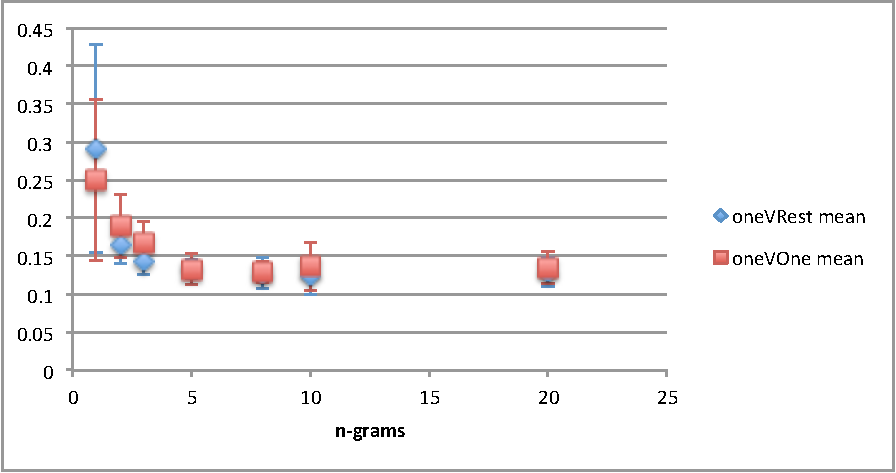
\includegraphics{n-grams.pdf}
  \caption{Tuning the length $n$ of sequences of system calls. Y-axis is error.}
\end{figure}

\begin{figure}
  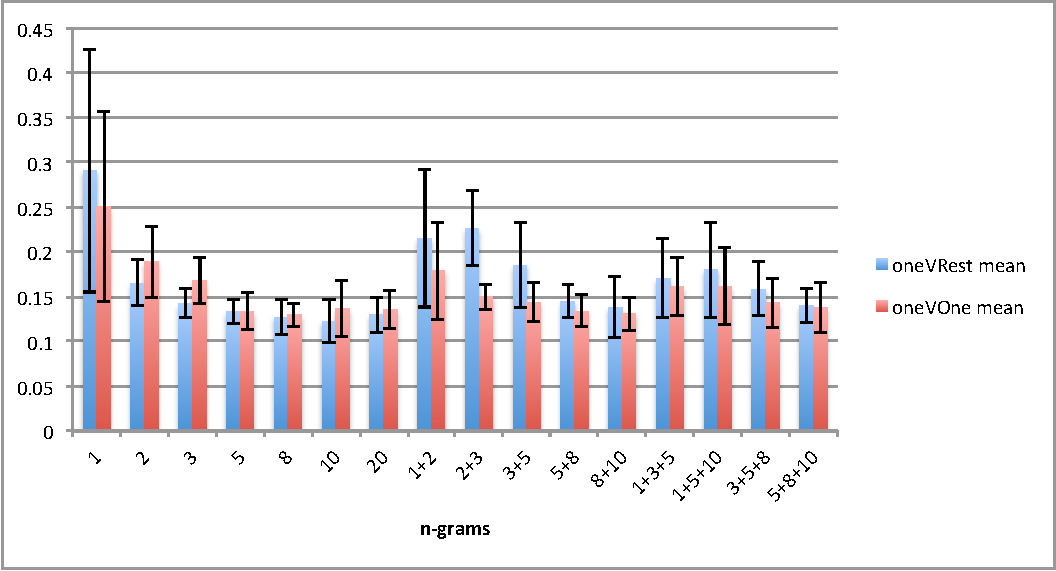
\includegraphics{n-grams-combos.pdf}
  \caption{Considering combinations of $n$-grams of system calls. Y-axis is error.}
\end{figure}

\begin{figure}
  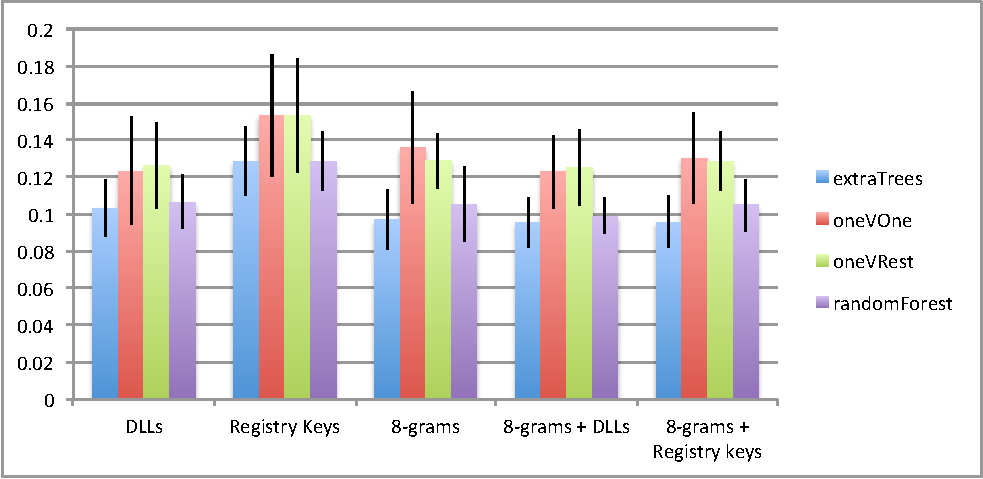
\includegraphics{other_features.pdf}
  \caption{Comparison of best-performing features. Y-axis is error.}
\end{figure}

\begin{figure}
  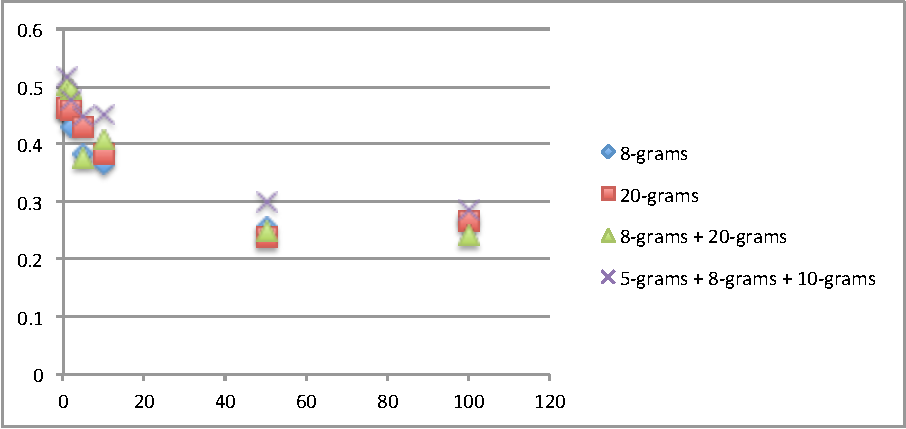
\includegraphics{tsvd.pdf}
  \caption{Comparison of a truncated singular value decomposition (TSVD) on various combinations of $n$-grams. The TSVD performed considerably worse than the full feature set in cross-validation, so it was not pursued.}
\end{figure}


\subsection{Classification Methods}



% -----------------------------------------------------------------------------
\section{Conclusion}


% -----------------------------------------------------------------------------
\begingroup
\begin{thebibliography}{9}

\bibitem{LSMR}
Fong, David Chin-Lung, and Michael Saunders. "LSMR: An iterative algorithm for sparse least-squares problems."
\emph{SIAM Journal on Scientific Computing} 33.5 (2011): 2950-2971

\end{thebibliography}
\endgroup

\end{document}